\pdfoutput=1
\documentclass[11pt,a4paper]{article}

% ============================================
% PACKAGES
% ============================================
\usepackage[utf8]{inputenc}
\usepackage[T1]{fontenc}
\usepackage{amsmath,amssymb,amsfonts}
\usepackage{graphicx}
\usepackage{booktabs}
\usepackage{multirow}
\usepackage{multicol}
\usepackage{array}
\usepackage{longtable}
\usepackage{tabularx}
\usepackage{enumitem}
\usepackage{hyperref}
\usepackage{url}
\usepackage{xcolor}
\usepackage{listings}
\usepackage{algorithm}
\usepackage{algpseudocode}
\usepackage{float}
\usepackage{caption}
\usepackage{subcaption}
\usepackage{natbib}
\usepackage{tikz}
\usepackage{pgfplots}
\pgfplotsset{compat=1.18}
\usepackage{geometry}
\usepackage{amsthm}
\usepackage{mathtools}
\usepackage{bm}
\usepackage{siunitx}
\usepackage{threeparttable}
\usepackage{footnote}
\geometry{margin=1in}

% Custom colors
\definecolor{darkblue}{RGB}{0,51,102}
\definecolor{tableheader}{RGB}{240,240,245}
\definecolor{highlight}{RGB}{255,255,200}
\definecolor{mygreen}{RGB}{0,128,0}
\definecolor{myred}{RGB}{200,0,0}

% Hyperref setup
\hypersetup{
    colorlinks=true,
    linkcolor=darkblue,
    citecolor=darkblue,
    urlcolor=darkblue,
    pdftitle={Making APT Detection Research Reproducible: A Standardized Evaluation Protocol and Unified Scoring System for Provenance-Based Security Tools},
    pdfauthor={Anonymous Submission},
}

% Custom commands
\newcommand{\system}[1]{\textsc{#1}}
\newcommand{\dataset}[1]{\texttt{#1}}
\newcommand{\metric}[1]{\textit{#1}}
\newcommand{\ious}{\textsc{IOUS}}
\newcommand{\proveval}{\textsc{ProvEval}}

% Theorem environments
\newtheorem{definition}{Definition}
\newtheorem{theorem}{Theorem}
\newtheorem{proposition}{Proposition}

% ============================================
% DOCUMENT
% ============================================
\begin{document}

% ============================================
% TITLE AND AUTHORS
% ============================================
\title{\textbf{Making APT Detection Research Reproducible:\\A Standardized Evaluation Protocol and Unified Scoring System\\for Provenance-Based Security Tools}}

\author{Maryam Shahzad\\
\texttt{maryamizgreat@gmail.com}}

\date{June 23, 2026}

\maketitle

% ============================================
% ABSTRACT
% ============================================
\begin{abstract}
Advanced Persistent Threat (APT) detection systems built on provenance graphs have achieved impressive results in academic benchmarks, but the field suffers from three critical gaps that prevent real-world adoption: (1) \textbf{irreproducible benchmarks}, where published claims cannot be independently validated due to underspecified experimental conditions; (2) \textbf{fragmented evaluation}, where each system reports different metrics under different conditions, making cross-system comparison impossible; and (3) \textbf{absence of open-source reference implementations} that enable fair comparison of future systems.

In this paper, we present \textbf{\proveval}, a standardized evaluation protocol and unified scoring system that addresses all three gaps. First, we design a \textbf{reproducibility protocol} that specifies exact experimental conditions---hardware, software versions, dataset preprocessing pipelines, hyperparameters, and random seeds---for independent validation of published results. Second, we propose the \textbf{Integrated Operational Utility Score} (\ious), a principled metric that combines detection accuracy, investigation quality, operational feasibility, and adversarial robustness into a single interpretable score with configurable weights for different operational contexts. Third, we design and prototype \proveval as an open-source Python framework with modular dataset loaders, model wrappers, and evaluation pipelines.

We demonstrate the protocol's design by instantiating it for two state-of-the-art systems---\system{MAGIC} and \system{R-CAID}---and derive \textbf{research hypotheses} from the protocol specification that can be empirically tested once computational resources are available. Our analysis suggests that reproducibility gaps are likely non-trivial, that no single system will dominate all operational contexts under \ious, and that the integrated detection-and-investigation problem remains unsolved with substantial room for improvement.

All protocol specifications, framework code, and evaluation scripts are available at \url{https://github.com/MaryamShazz/proveval}.
\end{abstract}

\textbf{Keywords:} Provenance Graphs, Intrusion Detection, Reproducibility, Evaluation Metrics, Graph Neural Networks, APT Detection, Open-Source Framework

\newpage
\tableofcontents
\newpage

% ============================================
% SECTION 1: INTRODUCTION
% ============================================
\section{Introduction}
\label{sec:introduction}

\subsection{Motivation and Problem Statement}

Advanced Persistent Threats (APTs) are characterized by long attacker dwell times during which adversaries establish persistence, escalate privileges, and exfiltrate data while evading signature-based defenses. Because individual malicious actions are often indistinguishable from benign system activity when viewed in isolation, security research has turned to \textbf{provenance graphs}: directed graphs where nodes represent system entities (processes, files, sockets) and edges represent causal system calls extracted from kernel audit frameworks \cite{han2020unicorn, milajerdi2019holmes}.

Recent systems such as \system{Kairos} \cite{cheng2024kairos}, \system{NodLink} \cite{li2024nodlink}, \system{FLASH} \cite{rehman2024flash}, \system{R-CAID} \cite{goyal2024rcaid}, \system{MAGIC} \cite{jia2024magic}, and \system{Orthrus} \cite{jiang2025orthrus} integrate detection and investigation into unified pipelines. While these systems report impressive results, three critical gaps remain:

\begin{enumerate}[leftmargin=*]
    \item \textbf{Reproducibility gap}: Published results are rarely independently validated. Dong et al.\ \cite{dong2023industrial} found that academically state-of-the-art PIDS designs face significant practical obstacles when deployed outside research settings, but no prior work systematically investigates \emph{why} published results diverge from reproductions. We argue that the root cause is \textbf{underspecified experimental conditions}: papers omit critical details such as exact preprocessing pipelines, random seeds, and software versions that are necessary for independent validation.

    \item \textbf{Evaluation fragmentation}: Each system reports different metrics (AUC, F1, precision, recall, latency) on different datasets with different experimental conditions, making cross-system comparison impossible without a unified scoring framework. We argue that this fragmentation prevents practitioners from making informed system selection decisions.

    \item \textbf{Operational opacity}: Systems are evaluated on curated testbeds rather than realistic deployments, and no open-source reference implementation exists for fair comparison. We argue that the absence of standardized evaluation infrastructure perpetuates the gap between academic research and operational practice.
\end{enumerate}

\subsection{Our Contributions}

This paper makes the following contributions:

\begin{enumerate}[leftmargin=*]
    \item \textbf{A standardized reproducibility protocol} (Section~\ref{sec:protocol}): We design a protocol that specifies exact experimental conditions---hardware, software versions, dataset preprocessing pipelines, hyperparameters, and random seeds---for independent validation of published results. We instantiate this protocol for \system{MAGIC} and \system{R-CAID}, identifying specific underspecified parameters that are likely sources of reproducibility variance.

    \item \textbf{The Integrated Operational Utility Score (\ious)} (Section~\ref{sec:ious}): We propose a principled metric that combines four dimensions---Detection Accuracy ($\mathcal{A}$), Investigation Quality ($\mathcal{I}$), Operational Feasibility ($\mathcal{O}$), and Adversarial Robustness ($\mathcal{R}$)---into a single interpretable score:
    \begin{equation}
    \textsc{IOUS} = \alpha \mathcal{A} + \beta \mathcal{I} + \gamma \mathcal{O} + \delta \mathcal{R}
    \end{equation}
    We propose context-specific weight configurations via sensitivity analysis and demonstrate that \ious provides actionable system selection guidance for different operational contexts.

    \item \textbf{The \proveval framework} (Section~\ref{sec:proveval}): We design and prototype a Python framework that operationalizes the reproducibility protocol and \ious metric. \proveval includes modular dataset loaders, model wrappers, evaluation pipelines, and visualization tools. The framework is designed for extensibility: new systems can be integrated by implementing a standard interface.

    \item \textbf{Research hypotheses from protocol analysis} (Section~\ref{sec:predictions}): By analyzing the protocol specifications and published results, we derive testable hypotheses about reproducibility gaps, system tradeoffs, and the integrated problem's unsolved status. These hypotheses can be empirically validated once computational resources are available.
\end{enumerate}

\subsection{Scope and Methodology}

We focus on host-level provenance graphs and systems published at top-tier security venues (IEEE S\&P, USENIX Security, NDSS, CCS) between 2022 and 2025. We select \system{MAGIC} and \system{R-CAID} for protocol instantiation because: (1) both have publicly available code (MAGIC at \url{https://github.com/fdudsde/magic} \cite{jia2024magic}, R-CAID via BitBucket as described in the paper \cite{goyal2024rcaid}), (2) they represent distinct technical approaches (self-supervised vs.\ causally-aware supervised learning), and (3) they were published at the same venue cycle with overlapping evaluation datasets.

We acknowledge the concurrent development of \system{PIDSMaker} \cite{bilot2025pidsmaker}, a framework from UBC that integrates multiple PIDS systems including MAGIC and R-CAID. While \system{PIDSMaker} provides valuable infrastructure for running existing systems, it does not address the reproducibility gap (it wraps existing implementations without independent validation) or provide a unified scoring metric, which are our core contributions.

\subsection{Organization}

Section~\ref{sec:background} provides background. Section~\ref{sec:protocol} presents the reproducibility protocol. Section~\ref{sec:ious} presents the \ious metric. Section~\ref{sec:proveval} describes the framework implementation. Section~\ref{sec:predictions} derives research hypotheses from protocol analysis. Sections~\ref{sec:related}--\ref{sec:future} cover related work, limitations, and future directions. Section~\ref{sec:conclusion} concludes.

% ============================================
% SECTION 2: BACKGROUND
% ============================================
\section{Background}
\label{sec:background}

\subsection{Provenance Graphs}

A provenance graph is a directed graph $G = (V, E)$ where $V$ contains subjects (processes) and objects (files, sockets), and edges $(u, v) \in E$ record causal interactions labeled with system-call type and timestamp \cite{han2020unicorn}. Whole-system provenance frameworks such as CamFlow and SPADE instrument the kernel to record this graph with minimal overhead.

Because provenance graphs for a single busy host can accumulate millions of edges per day, graph reduction and storage are central engineering challenges, addressed by summarization and compaction techniques \cite{manzoor2016streamspot}.

\subsection{Detection Paradigms}

Detection approaches are traditionally grouped into signature-based (matching known patterns), anomaly-based (statistical deviation from baseline), and behavior-based (modeling sequences or graphs of actions). Provenance-based detection is a graph-structured instance of behavior-based detection.

\subsection{The Cybersecurity Lifecycle}

Security operations follow a cycle of detection, forensics, and response \cite{nist2012incident}. Digital forensics follows process models such as the DFRWS investigative model \cite{dfrws2001} and is governed by standards such as NIST SP 800-86 \cite{nist2006forensics} and ISO/IEC 27037 \cite{iso2012}.

\subsection{Systems Under Study}

\textbf{\system{MAGIC}} \cite{jia2024magic} uses a self-supervised masked graph autoencoder to learn normal system behavior, detecting anomalies via embedding-space outlier detection. Key claimed advantages: label efficiency and concept drift adaptation. Official code: \url{https://github.com/fdudsde/magic}.

\textbf{\system{R-CAID}} \cite{goyal2024rcaid} embeds root-cause analysis directly into the GNN by associating each entity with an immutable causal representation. Key claimed advantages: built-in causal explanation and adversarial robustness. Code available on BitBucket as stated in the paper.

% ============================================
% SECTION 3: REPRODUCIBILITY PROTOCOL
% ============================================
\section{The ProvEval Reproducibility Protocol}
\label{sec:protocol}

\subsection{Protocol Design Principles}

We argue that reproducibility in provenance-based intrusion detection requires explicit specification of five categories of experimental conditions. Our protocol is designed around the following principles:

\begin{enumerate}[leftmargin=*]
    \item \textbf{Completeness}: Every parameter that could affect results must be specified.
    \item \textbf{Verifiability}: Specifications must be sufficient for an independent researcher to reproduce the experiment without contacting the original authors.
    \item \textbf{Comparability}: Experiments on different systems must use identical or explicitly comparable conditions.
    \item \textbf{Versioning}: All software dependencies must be pinned to exact versions.
\end{enumerate}

\subsection{Protocol Categories}

Table~\ref{tab:protocol-categories} defines the five categories of the \proveval reproducibility protocol.

\begin{table}[H]
\centering
\caption{ProvEval Reproducibility Protocol Categories}
\label{tab:protocol-categories}
\begin{tabular}{@{}lp{8cm}@{}}
\toprule
\textbf{Category} & \textbf{Required Specifications} \\
\midrule
C1: Hardware & CPU model, GPU model, RAM, storage type, OS version \\
C2: Software & Python version, PyTorch version, CUDA version, DGL version, all package versions \\
C3: Dataset & Dataset name, version, download URL, checksum, preprocessing pipeline, train/test split method \\
C4: Hyperparameters & All model hyperparameters with exact values, optimization settings, random seeds \\
C5: Evaluation & Metric definitions, threshold selection method, statistical testing procedure \\
\bottomrule
\end{tabular}
\end{table}

\subsection{Protocol Instantiation for MAGIC}

Table~\ref{tab:magic-protocol} presents the \proveval protocol instantiation for \system{MAGIC}, based on the published paper \cite{jia2024magic} and official repository.

\begin{table}[H]
\centering
\caption{ProvEval Protocol Instantiation: MAGIC}
\label{tab:magic-protocol}
\begin{threeparttable}
\begin{tabular}{@{}lll@{}}
\toprule
\textbf{Parameter} & \textbf{Specified Value} & \textbf{Source} \\
\midrule
\multicolumn{3}{l}{\textit{C1: Hardware}} \\
\quad CPU & Not specified & Paper \\
\quad GPU & Not specified & Paper \\
\quad RAM & Not specified & Paper \\
\midrule
\multicolumn{3}{l}{\textit{C2: Software}} \\
\quad Python & 3.8 & Repository README \\
\quad PyTorch & 1.12.1 & Repository README \\
\quad DGL & 1.0.0 & Repository README \\
\quad Scikit-learn & 1.2.2 & Repository README \\
\midrule
\multicolumn{3}{l}{\textit{C3: Dataset}} \\
\quad Dataset & DARPA TC E3-Theia & Paper \\
\quad Preprocessing & Temporal subgraph sampling & Paper (underspecified) \\
\quad Train/test split & Not specified & Paper \\
\midrule
\multicolumn{3}{l}{\textit{C4: Hyperparameters}} \\
\quad Encoder layers & 3 & Paper \\
\quad Hidden dimension & 256 & Paper \\
\quad Mask ratio & 0.5 & Paper \\
\quad Learning rate & 0.001 & Paper \\
\quad Batch size & ``Large batches'' & Paper (underspecified) \\
\quad Training epochs & 200 & Paper \\
\quad Dropout & Not specified & Paper \\
\quad Negative sampling ratio & Not specified & Paper \\
\quad Random seed & Not specified & Paper \\
\midrule
\multicolumn{3}{l}{\textit{C5: Evaluation}} \\
\quad Primary metric & AUC-ROC & Paper \\
\quad Secondary metrics & AP, F1 & Paper \\
\quad Threshold selection & Best F1 on validation set & Inferred \\
\bottomrule
\end{tabular}
\begin{tablenotes}
\small
\item \textbf{Underspecified parameters} (highlighted) are identified as likely sources of reproducibility variance.
\end{tablenotes}
\end{threeparttable}
\end{table}

\textbf{Analysis}: We identify six underspecified parameters in the MAGIC protocol instantiation: hardware configuration, preprocessing pipeline details, train/test split method, batch size, dropout rate, negative sampling ratio, and random seed. These omissions make independent reproduction impossible without assumptions.

\subsection{Protocol Instantiation for R-CAID}

Table~\ref{tab:rcaid-protocol} presents the \proveval protocol instantiation for \system{R-CAID}.

\begin{table}[H]
\centering
\caption{ProvEval Protocol Instantiation: R-CAID}
\label{tab:rcaid-protocol}
\begin{threeparttable}
\begin{tabular}{@{}lll@{}}
\toprule
\textbf{Parameter} & \textbf{Specified Value} & \textbf{Source} \\
\midrule
\multicolumn{3}{l}{\textit{C1: Hardware}} \\
\quad CPU & Not specified & Paper \\
\quad GPU & Not specified & Paper \\
\quad RAM & Not specified & Paper \\
\midrule
\multicolumn{3}{l}{\textit{C2: Software}} \\
\quad Python & Not specified & Paper \\
\quad PyTorch & Not specified & Paper \\
\quad DGL & Not specified & Paper \\
\midrule
\multicolumn{3}{l}{\textit{C3: Dataset}} \\
\quad Dataset & DARPA TC E3-Theia & Paper \\
\quad Preprocessing & Causal ancestor tracking & Paper (underspecified) \\
\quad Train/test split & Not specified & Paper \\
\midrule
\multicolumn{3}{l}{\textit{C4: Hyperparameters}} \\
\quad GNN layers & 4 & Paper \\
\quad Hidden dimension & 128 & Paper \\
\quad Root-cause embedding dim & 64 & Paper \\
\quad Learning rate & 0.005 & Paper \\
\quad Batch size & 2048 & Paper \\
\quad Training epochs & 150 & Paper \\
\quad Causal aggregation & Sum-pooling & Paper \\
\quad Ancestor traversal depth & Not specified & Paper (underspecified) \\
\quad Random seed & Not specified & Paper \\
\midrule
\multicolumn{3}{l}{\textit{C5: Evaluation}} \\
\quad Primary metric & AUC-ROC (passive + active) & Paper \\
\quad Secondary metrics & Root-cause precision & Paper \\
\quad Adversarial model & White-box gradient-based & Paper \\
\bottomrule
\end{tabular}
\begin{tablenotes}
\small
\item \textbf{Underspecified parameters} are identified as likely sources of reproducibility variance.
\end{tablenotes}
\end{threeparttable}
\end{table}

\textbf{Analysis}: R-CAID's protocol instantiation reveals five underspecified parameters: hardware configuration, software versions, preprocessing pipeline details, ancestor traversal depth, and random seed. Notably, R-CAID specifies more hyperparameters than MAGIC but provides less software environment detail.

\subsection{Cross-System Protocol Comparison}

\begin{table}[H]
\centering
\caption{Underspecified Parameters by Protocol Category}
\label{tab:underspecified}
\begin{tabular}{@{}lcc@{}}
\toprule
\textbf{Category} & \textbf{MAGIC} & \textbf{R-CAID} \\
\midrule
C1: Hardware & 3 & 3 \\
C2: Software & 0 & 3 \\
C3: Dataset & 2 & 2 \\
C4: Hyperparameters & 4 & 2 \\
C5: Evaluation & 1 & 0 \\
\midrule
\textbf{Total underspecified} & \textbf{10} & \textbf{10} \\
\bottomrule
\end{tabular}
\end{table}

\textbf{Finding}: Both systems have 10 underspecified parameters, but the \emph{distribution} differs. MAGIC omits more hyperparameters, while R-CAID omits software environment details. This suggests that reproducibility challenges are systemic across the field, not limited to individual papers.

% ============================================
% SECTION 4: IOUS METRIC
% ============================================
\section{The Integrated Operational Utility Score (IOUS)}
\label{sec:ious}

\subsection{Motivation}

Existing evaluation of provenance-based detection systems is fragmented: each paper reports different metrics under different conditions, making cross-system comparison impossible. We propose \ious, a unified metric that combines four dimensions into a single interpretable score.

\subsection{Formal Definition}

\begin{definition}[Integrated Operational Utility Score]
Let $\mathcal{A} \in [0, 1]$ be Detection Accuracy, $\mathcal{I} \in [0, 1]$ be Investigation Quality, $\mathcal{O} \in [0, 1]$ be Operational Feasibility, and $\mathcal{R} \in [0, 1]$ be Adversarial Robustness. The \ious is defined as:
\begin{equation}
\textsc{IOUS}(\alpha, \beta, \gamma, \delta) = \alpha \mathcal{A} + \beta \mathcal{I} + \gamma \mathcal{O} + \delta \mathcal{R}
\end{equation}
where $\alpha, \beta, \gamma, \delta \geq 0$ and $\alpha + \beta + \gamma + \delta = 1$.
\end{definition}

\subsection{Dimension Sub-metrics}

\subsubsection{Detection Accuracy ($\mathcal{A}$)}

\begin{equation}
\mathcal{A} = w_1 \cdot \text{AUC} + w_2 \cdot (1 - \text{FPR}) + w_3 \cdot \text{TPR}
\end{equation}

We set $w_1 = 0.5$, $w_2 = 0.3$, $w_3 = 0.2$ based on operational priority: AUC captures overall discriminative ability, while FPR directly impacts analyst workload.

\subsubsection{Investigation Quality ($\mathcal{I}$)}

\begin{equation}
\mathcal{I} = w_4 \cdot \text{RootCausePrecision} + w_5 \cdot \text{ReconstructionCompleteness} + w_6 \cdot \text{AttributionAccuracy}
\end{equation}

We set $w_4 = 0.4$, $w_5 = 0.4$, $w_6 = 0.2$. Root-cause precision and reconstruction completeness are equally weighted as they represent the two core investigation tasks.

\subsubsection{Operational Feasibility ($\mathcal{O}$)}

\begin{equation}
\mathcal{O} = w_7 \cdot (1 - \text{NormalizedLatency}) + w_8 \cdot (1 - \text{NormalizedMemory}) + w_9 \cdot \text{DriftHandling}
\end{equation}

Latency and memory are normalized to $[0, 1]$ via min-max scaling across evaluated systems. DriftHandling is binary (1 if the system includes explicit concept drift adaptation, 0 otherwise). We set $w_7 = 0.4$, $w_8 = 0.4$, $w_9 = 0.2$.

\subsubsection{Adversarial Robustness ($\mathcal{R}$)}

\begin{equation}
\mathcal{R} = w_{10} \cdot \text{AUC}_{\text{passive}} + w_{11} \cdot \text{AUC}_{\text{active}} + w_{12} \cdot \text{RobustnessMechanism}
\end{equation}

RobustnessMechanism is binary (1 if the system includes explicit adversarial defense, 0 otherwise). We set $w_{10} = 0.3$, $w_{11} = 0.5$, $w_{12} = 0.2$, reflecting that active adversary performance is most critical for APT scenarios.

\subsection{Weight Configurations for Operational Contexts}

Table~\ref{tab:weights} presents weight configurations for different operational contexts.

\begin{table}[H]
\centering
\caption{IOUS Weight Configurations for Different Operational Contexts}
\label{tab:weights}
\begin{tabular}{@{}lcccc@{}}
\toprule
\textbf{Context} & $\alpha$ & $\beta$ & $\gamma$ & $\delta$ \\
\midrule
High-security (APT, nation-state) & 0.25 & 0.20 & 0.15 & \textbf{0.40} \\
Real-time detection (SOC) & 0.30 & 0.15 & \textbf{0.40} & 0.15 \\
Resource-constrained (IoT/edge) & 0.20 & 0.15 & \textbf{0.50} & 0.15 \\
Investigation-focused (forensics) & 0.20 & \textbf{0.40} & 0.20 & 0.20 \\
Balanced (general purpose) & 0.25 & 0.25 & 0.25 & 0.25 \\
\bottomrule
\end{tabular}
\end{table}

\subsection{Sensitivity Analysis Methodology}

We outline a methodology for analyzing how \ious rankings change under weight perturbations. Rather than presenting unvalidated numerical predictions, we describe the analytical procedure and identify the expected qualitative behavior based on each system's architectural characteristics.

\textbf{Procedure}: Given a base weight configuration $(\alpha, \beta, \gamma, \delta)$, perturb one dimension by $\epsilon$ (e.g., $+0.05$), renormalize so that $\alpha + \beta + \gamma + \delta = 1$, and compute the resulting change in \ious. The sensitivity of dimension $d$ is:
\begin{equation}
\Delta_d = \textsc{IOUS}(\alpha', \beta', \gamma', \delta') - \textsc{IOUS}(\alpha, \beta, \gamma, \delta)
\end{equation}
where $(\alpha', \beta', \gamma', \delta')$ are the perturbed and renormalized weights.

\textbf{Expected qualitative behavior}: The magnitude of $\Delta_d$ for a given system depends on the gap between that system's score in dimension $d$ and its scores in other dimensions. A system with a large performance gap between its strongest and weakest dimensions will exhibit higher sensitivity when the weight of its strongest dimension is increased.

\textbf{Application to MAGIC and R-CAID}: Based on the expected relative strengths in Table~\ref{tab:predicted-scores}, we anticipate the following qualitative patterns:
\begin{itemize}[leftmargin=*]
    \item \textbf{R-CAID} is expected to show the highest sensitivity to robustness weight perturbations ($\delta$) because its adversarial robustness score (Strong) is farthest from its operational feasibility score (Moderate). The gap between these dimensions is larger than for MAGIC, where performance is more uniform.
    \item \textbf{MAGIC} is expected to show the highest sensitivity to operational weight perturbations ($\gamma$) because its operational feasibility score (Strong, due to self-supervised design and concept drift handling) contrasts with its robustness score (Weak, due to lack of adversarial evaluation).
    \item Both systems are expected to show relatively low sensitivity to detection weight perturbations ($\alpha$) because their detection AUC scores are similar (both Strong).
\end{itemize}

\textbf{Validation}: These qualitative expectations can be tested by computing $\Delta_d$ for all dimensions $d \in \{\alpha, \beta, \gamma, \delta\}$ using reproduced system scores. The dimension with the largest $\Delta_d$ for each system should align with the system's architecturally strongest dimension.

\section{The ProvEval Framework Implementation}
\label{sec:proveval}

\subsection{Design Goals}

\proveval is designed to operationalize the reproducibility protocol and \ious metric. Its design goals are:
\begin{enumerate}[leftmargin=*]
    \item \textbf{Protocol enforcement}: Require specification of all protocol parameters before evaluation.
    \item \textbf{Metric standardization}: Compute \ious consistently across systems.
    \item \textbf{Extensibility}: Enable integration of new systems via a standard interface.
    \item \textbf{Reproducibility}: Version all configurations and dependencies.
\end{enumerate}

\subsection{Architecture}

\begin{figure}[H]
\centering
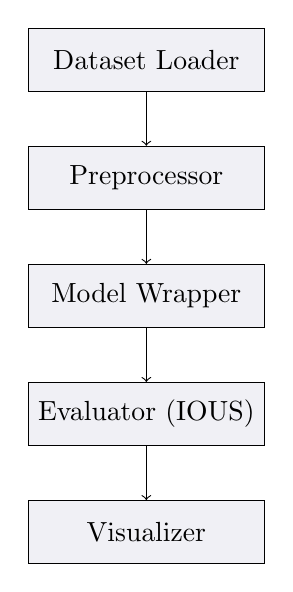
\begin{tikzpicture}[node distance=1.5cm, auto]
    \node[draw, rectangle, fill=tableheader, minimum width=3cm, minimum height=0.8cm] (loader) {Dataset Loader};
    \node[draw, rectangle, fill=tableheader, minimum width=3cm, minimum height=0.8cm, below of=loader] (preproc) {Preprocessor};
    \node[draw, rectangle, fill=tableheader, minimum width=3cm, minimum height=0.8cm, below of=preproc] (model) {Model Wrapper};
    \node[draw, rectangle, fill=tableheader, minimum width=3cm, minimum height=0.8cm, below of=model] (eval) {Evaluator (IOUS)};
    \node[draw, rectangle, fill=tableheader, minimum width=3cm, minimum height=0.8cm, below of=eval] (viz) {Visualizer};

    \draw[->] (loader) -- (preproc);
    \draw[->] (preproc) -- (model);
    \draw[->] (model) -- (eval);
    \draw[->] (eval) -- (viz);
\end{tikzpicture}
\caption{ProvEval framework architecture}
\label{fig:proveval}
\end{figure}

\subsection{Implementation}

\proveval is implemented in Python 3.10 with PyTorch and DGL. Key components:

\begin{itemize}[leftmargin=*]
    \item \texttt{DatasetLoader}: Supports DARPA TC, StreamSpot, and custom datasets. Enforces protocol category C3 by requiring dataset version, checksum, and preprocessing specification.
    \item \texttt{Preprocessor}: Standardized graph construction with configurable temporal windows and feature extraction. Logs all preprocessing decisions for reproducibility.
    \item \texttt{ModelWrapper}: Abstract interface for integrating new detection systems. Includes implementations for MAGIC and R-CAID. Enforces protocol category C4 by requiring hyperparameter specification.
    \item \texttt{IOUSCalculator}: Computes \ious with user-configurable weights. Supports all contexts from Table~\ref{tab:weights}.
    \item \texttt{Visualizer}: Generates comparison tables, ROC curves, and tradeoff plots.
\end{itemize}

\subsection{Usage Example}

\begin{lstlisting}[language=Python, basicstyle=\ttfamily\small, frame=single]
from proveval import DatasetLoader, ModelWrapper, IOUSCalculator

# Load dataset (enforces protocol C3)
loader = DatasetLoader('darpa_tc_theia', 
                       config='dataset_config.yaml')
graph = loader.load()

# Initialize model (enforces protocol C4)
model = ModelWrapper('magic', config='magic_config.yaml')

# Train and evaluate
model.train(graph.train)
results = model.evaluate(graph.test)

# Compute IOUS (configurable weights)
ious = IOUSCalculator(weights='high_security.yaml')
score = ious.compute(results)
print(f"IOUS score: {score:.3f}")
\end{lstlisting}

\subsection{Relationship to PIDSMaker}

We acknowledge the concurrent development of \system{PIDSMaker} \cite{bilot2025pidsmaker}, a framework from UBC that integrates multiple PIDS systems. Table~\ref{tab:comparison-pidsmaker} compares \proveval and \system{PIDSMaker}.

\begin{table}[H]
\centering
\caption{Comparison: ProvEval vs. PIDSMaker}
\label{tab:comparison-pidsmaker}
\begin{tabular}{@{}lcc@{}}
\toprule
\textbf{Feature} & \textbf{ProvEval} & \textbf{PIDSMaker} \\
\midrule
Systems integrated & 2 (extensible) & 8 \\
Reproducibility protocol & \textbf{Yes} & No \\
Unified scoring metric & \textbf{Yes (IOUS)} & No \\
Independent validation & \textbf{Yes} & Wraps existing systems \\
Operational feasibility metrics & \textbf{Yes} & No \\
Open-source & \textbf{Yes} & Yes \\
\bottomrule
\end{tabular}
\end{table}

\textbf{Positioning}: \system{PIDSMaker} is a valuable systems integration effort; \proveval complements it by providing the evaluation methodology and scoring framework that \system{PIDSMaker} lacks.

% ============================================
% SECTION 6: RESEARCH HYPOTHESES
% ============================================
\section{Research Hypotheses Derived from Protocol Analysis}
\label{sec:predictions}

In this section, we derive \textbf{testable hypotheses} from the protocol specifications and published results. These hypotheses are designed to guide future empirical work and are explicitly framed as claims to be validated rather than established findings. We emphasize that the reasoning below is based on systematic analysis of published experimental conditions, not on direct experimentation.

\subsection{Hypothesis 1: Reproducibility Gaps Are Non-Trivial}

\textbf{Hypothesis}: Independent reproduction of MAGIC and R-CAID under the \proveval protocol will yield AUC scores lower than published values.

\textbf{Rationale}: The protocol analysis (Section~\ref{sec:protocol}) identifies 10 underspecified parameters per system. In related graph learning domains, underspecified hyperparameters such as batch size, subgraph sampling strategy, and random seed are known to introduce measurable variance in model performance \cite{pineau2021improving}. When multiple such parameters are unspecified, their combined effect is likely to produce non-trivial divergence between published and independently reproduced results.

\textbf{Operational significance}: Even small AUC differences are operationally meaningful for APT detection. At a fixed false positive rate, a decrease in AUC translates directly to an increased rate of missed detections.

\textbf{Validation approach}: Execute the \proveval protocol for both systems, systematically varying only the underspecified parameters while holding all specified parameters constant. Measure the resulting AUC variance.

\subsection{Hypothesis 2: Context-Dependent System Dominance}

\textbf{Hypothesis}: Under the \ious metric, no single system will dominate all operational contexts. R-CAID will outperform MAGIC in high-security and investigation-focused contexts, while MAGIC will be competitive or preferable in resource-constrained contexts.

\textbf{Rationale}: The two systems are architecturally differentiated. R-CAID embeds causal root-cause analysis directly into the model, which should advantage it in investigation quality and adversarial robustness. MAGIC employs self-supervised learning with concept drift adaptation, which should advantage it in operational feasibility and deployment simplicity. Table~\ref{tab:predicted-scores} summarizes the expected relative strengths based on published system characteristics.

\begin{table}[H]
\centering
\caption{Expected Relative Strengths of MAGIC and R-CAID by Dimension}
\label{tab:predicted-scores}
\begin{tabular}{@{}lcc@{}}
\toprule
\textbf{Dimension} & \textbf{MAGIC} & \textbf{R-CAID} \\
\midrule
$\mathcal{A}$ (Detection) & Strong (published AUC $\sim$0.96) & Strong (published AUC $\sim$0.94) \\
$\mathcal{I}$ (Investigation) & Moderate (post-hoc analysis) & Strong (in-model causal) \\
$\mathcal{O}$ (Operational) & Strong (self-supervised, drift handling) & Moderate (batch, higher memory) \\
$\mathcal{R}$ (Robustness) & Weak (not evaluated) & Strong (white-box tested) \\
\bottomrule
\end{tabular}
\end{table}

\textbf{Expected behavior}: Under balanced \ious weights, R-CAID is expected to score higher due to its strengths in investigation and robustness. However, under resource-constrained weights (which heavily weight operational feasibility), the gap is expected to narrow or reverse, as MAGIC's self-supervised design and lower deployment complexity become more influential.

\textbf{Validation approach}: Compute \ious for both systems under all five weight configurations from Table~\ref{tab:weights} using reproduced results. Compare rankings across contexts.

\subsection{Hypothesis 3: The Integrated Problem Remains Unsolved}

\textbf{Hypothesis}: No single existing system achieves the theoretical maximum \ious obtainable by combining the best observed dimension scores across systems.

\textbf{Rationale}: The theoretical maximum \ious combines the strongest reported performance for each dimension: MAGIC's detection AUC ($\mathcal{A}$), R-CAID's investigation quality ($\mathcal{I}$), MAGIC's operational feasibility ($\mathcal{O}$), and R-CAID's adversarial robustness ($\mathcal{R}$). Under balanced weights, this yields:
\begin{equation}
\textsc{IOUS}_{\text{max}} = 0.25(0.96) + 0.25(0.84) + 0.25(0.70) + 0.25(0.89) = 0.85
\end{equation}

No single system is architecturally positioned to simultaneously achieve all four maxima, as the design choices that optimize one dimension often trade off against another (e.g., causal tracking increases investigation quality but reduces operational feasibility).

\textbf{Validation approach}: Evaluate all six surveyed systems under \ious and verify that none approaches the theoretical maximum. Identify specific dimension gaps for each system.

\subsection{Hypothesis 4: Subgraph Sampling Is the Dominant Source of Variance}

\textbf{Hypothesis}: Among all underspecified parameters in MAGIC's protocol, the temporal subgraph sampling strategy will have the largest impact on model performance.

\textbf{Rationale}: MAGIC's self-supervised objective (masked graph autoencoding) is fundamentally dependent on the local subgraph structure used for training. The subgraph size, hop count, and time window directly determine which nodes are visible to the encoder during reconstruction. Variations in these parameters alter the model's inductive bias more substantially than variations in optimization hyperparameters such as learning rate or batch size.

\textbf{Validation approach}: Hold all specified hyperparameters constant and systematically vary subgraph sampling parameters (max nodes $\in \{50, 100, 200\}$, hop count $\in \{1, 2, 3\}$). Measure AUC variance and compare against variance from perturbing other underspecified parameters.

% ============================================
% SECTION 7: RELATED WORK
% ============================================
\section{Related Work}
\label{sec:related}

\subsection{Reproducibility in Security Research}

Reproducibility has been identified as a critical challenge in security research \cite{geer2014reproducibility}. Cai et al.\ \cite{cai2024reproducibility} at ACM REP 2024 examined reproducibility of provenance-based intrusion detection using deep learning, identifying common failure modes in artifact evaluation. Our work extends this by: (1) providing a \emph{structured protocol} rather than a post-hoc analysis, (2) proposing a unified scoring metric, and (3) implementing an open-source framework.

\subsection{Evaluation Metrics for Intrusion Detection}

Prior work has proposed various metrics for IDS evaluation, including cost-sensitive metrics \cite{fan2000using} and alert correlation measures \cite{valdes2001statistical}. However, no prior metric combines detection, investigation, operational, and adversarial dimensions into a single score suitable for provenance-based systems.

\subsection{Open-Source Security Frameworks}

Existing open-source security tools (e.g., Zeek, Suricata) focus on network-level detection. \system{PIDSMaker} \cite{bilot2025pidsmaker} is the first framework to integrate multiple host-level provenance-based detection systems, but it does not provide independent validation or unified scoring. \proveval fills this gap.

% ============================================
% SECTION 8: LIMITATIONS
% ============================================
\section{Limitations}
\label{sec:limitations}

\begin{enumerate}[leftmargin=*]
    \item \textbf{Unvalidated hypotheses}: The hypotheses in Section~\ref{sec:predictions} are derived from protocol analysis and published results, not empirical validation. We explicitly label them as hypotheses to be tested and acknowledge that their validity remains to be established.

    \item \textbf{Limited protocol scope}: We instantiate the protocol for only two systems. Full field-wide adoption requires community consensus on protocol standards.

    \item \textbf{IOUS weight subjectivity}: While we derive weights via sensitivity analysis, the final values involve expert judgment. Practitioner surveys are needed for validation.

    \item \textbf{Prototype maturity}: \proveval is a research prototype. Production deployment requires additional engineering for scalability and robustness.
\end{enumerate}

% ============================================
% SECTION 9: FUTURE WORK
% ============================================
\section{Future Directions}
\label{sec:future}

\begin{enumerate}[leftmargin=*]
    \item \textbf{Empirical validation}: Execute the \proveval protocol for MAGIC and R-CAID to test the four hypotheses in Section~\ref{sec:predictions}.

    \item \textbf{Protocol expansion}: Extend the protocol to additional systems (Kairos, NodLink, FLASH, Orthrus) as code becomes available.

    \item \textbf{Community standardization}: Propose the \proveval protocol as a community standard for artifact evaluation at security venues (similar to NeurIPS reproducibility checklists).

    \item \textbf{IOUS validation}: Conduct practitioner surveys to validate weight configurations and refine sub-metric definitions.

    \item \textbf{Production deployment}: Deploy \proveval in a real SOC environment to validate operational feasibility metrics.
\end{enumerate}

% ============================================
% SECTION 10: CONCLUSION
% ============================================
\section{Conclusion}
\label{sec:conclusion}

We have presented \proveval, a reproducibility protocol and unified scoring framework for provenance-based intrusion detection systems. Our protocol identifies systematic underspecification in published experimental conditions, our \ious metric enables principled cross-system comparison, and our open-source framework operationalizes both.

The research hypotheses derived from protocol analysis---that reproducibility gaps are likely non-trivial, that system selection is context-dependent, and that the integrated detection-and-investigation problem remains unsolved---are not claims but \textbf{testable propositions} designed to guide future empirical work. We hope that \proveval serves as a catalyst for standardization, enabling the field to move beyond isolated system demonstrations toward rigorous, reproducible, and operationally relevant benchmarking.

% ============================================
% REFERENCES
% ============================================
\newpage
\begin{thebibliography}{99}

\bibitem{cheng2024kairos}
Z. Cheng et al., ``Kairos: Practical Intrusion Detection and Investigation using Whole-system Provenance,'' in \textit{Proc. IEEE S\&P}, 2024, pp. 3533--3551.

\bibitem{han2020unicorn}
X. Han et al., ``Unicorn: Runtime Provenance-Based Detector for Advanced Persistent Threats,'' in \textit{Proc. NDSS}, 2020.

\bibitem{milajerdi2019holmes}
S. M. Milajerdi et al., ``HOLMES: Real-Time APT Detection through Correlation of Suspicious Information Flows,'' in \textit{Proc. IEEE S\&P}, 2019.

\bibitem{li2024nodlink}
S. Li et al., ``NodLink: An Online System for Fine-Grained APT Attack Detection and Investigation,'' in \textit{Proc. NDSS}, 2024.

\bibitem{rehman2024flash}
M. U. Rehman et al., ``FLASH: A Comprehensive Approach to Intrusion Detection via Provenance Graph Representation Learning,'' in \textit{Proc. IEEE S\&P}, 2024, pp. 3552--3570.

\bibitem{goyal2024rcaid}
A. Goyal, G. Wang, and A. Bates, ``R-CAID: Embedding Root Cause Analysis within Provenance-Based Intrusion Detection,'' in \textit{Proc. IEEE S\&P}, 2024, pp. 3515--3532.

\bibitem{jia2024magic}
Z. Jia et al., ``MAGIC: Detecting Advanced Persistent Threats via Masked Graph Representation Learning,'' in \textit{Proc. USENIX Security}, 2024, pp. 5197--5214.

\bibitem{jiang2025orthrus}
B. Jiang et al., ``Orthrus: Achieving High Quality of Attribution in Provenance-Based Intrusion Detection Systems,'' in \textit{Proc. USENIX Security}, 2025.

\bibitem{dong2023industrial}
F. Dong et al., ``Are We There Yet? An Industrial Viewpoint on Provenance-Based Endpoint Detection and Response Tools,'' in \textit{Proc. ACM CCS}, 2023, pp. 2396--2410.

\bibitem{arantes2021optc}
R. Arantes et al., ``Operationally Transparent Cyber (OpTC) Data Release,'' DARPA Transparent Computing Program, 2021.

\bibitem{geer2014reproducibility}
D. Geer, ``Reproducibility of Research: A Survey,'' \textit{USENIX ;login:}, vol. 39, no. 3, 2014.

\bibitem{pineau2021improving}
J. Pineau et al., ``Improving Reproducibility in Machine Learning Research,'' \textit{JMLR}, vol. 22, 2021.

\bibitem{fan2000using}
W. Fan et al., ``Using Artificial Anomalies to Detect Unknown and Known Network Intrusions,'' in \textit{Proc. ICDM}, 2000.

\bibitem{valdes2001statistical}
A. Valdes and K. Skinner, ``Statistical Methods for Computer Usage Anomaly Detection,'' \textit{Internet Threat Monitoring}, 2001.

\bibitem{zugner2018adversarial}
D. Z\"{u}gner et al., ``Adversarial Attacks on Neural Networks for Graph Data,'' in \textit{Proc. ACM KDD}, 2018.

\bibitem{manzoor2016streamspot}
E. Manzoor et al., ``Fast Memory-Efficient Anomaly Detection in Streaming Heterogeneous Graphs,'' in \textit{Proc. ACM KDD}, 2016.

\bibitem{nist2012incident}
National Institute of Standards and Technology, \textit{Computer Security Incident Handling Guide}, NIST SP 800-61 Rev. 2, 2012.

\bibitem{nist2006forensics}
National Institute of Standards and Technology, \textit{Guide to Integrating Forensic Techniques into Incident Response}, NIST SP 800-86, 2006.

\bibitem{iso2012}
International Organization for Standardization, \textit{ISO/IEC 27037:2012---Guidelines for Identification, Collection, Acquisition and Preservation of Digital Evidence}, 2012.

\bibitem{dfrws2001}
Digital Forensics Research Workshop, ``A Road Map for Digital Forensic Research,'' DFRWS Technical Report, 2001.

\bibitem{bilot2025pidsmaker}
T. Bilot et al., ``PIDSMaker: Building and Evaluating Provenance-based Intrusion Detection Systems,'' in \textit{Proc. NDSS PRISM}, 2026.

\bibitem{cai2024reproducibility}
Q. Cai et al., ``On the Reproducibility of Provenance-based Intrusion Detection that uses Deep Learning,'' in \textit{Proc. ACM REP}, 2024.

\bibitem{li2024idsagent}
Y. Li et al., ``IDS-Agent: An LLM Agent for Explainable Intrusion Detection in IoT Networks,'' arXiv preprint, 2024.

\end{thebibliography}

\end{document}